%\clearpage\setcounter{page}{43}
\thispagestyle{empty}
\phantomsection{}
\addcontentsline{toc}{chapter}{Programa de estudios con Línea Terminal\\ en Enseñanza de la Historia en la Universidad\\ Autónoma de Querétaro\newline $\diamond$
\normalfont\textit{Paulina Latapí Escalante}}
{\centering {\scshape \large Programa de estudios con línea terminal en enseñanza\\ de la historia en la Universidad Autónoma de Querétaro}\par}
\markboth{la formación del historiador}{el programa de estudios}
\setcounter{footnote}{0}

\bigskip
\begin{center}
%\begin{flushleft}
{\bfseries Paulina Latapí Escalante}\\
{\itshape\ Universidad Autónoma de Querétaro\/}
%\end{flushleft}
\end{center}

\bigskip
\noindent {\bfseries Resumen}


\noindent El presente trabajo da cuenta de los primeros pasos de la 
Línea Terminal en Enseñanza de la Historia de la licenciatura en 
Historia en la Universidad Autónoma de Querétaro. Para ello explica el 
diseño e inclusión  de la Línea Terminal en el plan de estudios 
vigente, así como su secuencia y articulación programática con base en 
los objetivos, las temáticas y las estrategias planteadas para cada 
asignatura. El análisis se realiza desde la perspectiva de la 
aplicación de un instrumento de diseño, desarrollo y evaluación 
curricular (mapa mental) y se apoya en los resultados de cuestionarios 
aplicados tanto a alumnas y alumnos de la primera generación como a 
docentes de la misma. Sobresale el énfasis que se ha dado a la 
investigación  sobre  enseñanza de la historia desde un enfoque 
interdisciplinario en el cual la vinculación social ha sido fundamental 
en el trabajo de las y los alumnos al desarrollar recursos didácticos 
para la solución de problemas de la disciplina de la historia en el 
aula como son los sujetos de la historia, el tiempo, el espacio  y la 
causalidad, principalmente en el nivel educativo básico y medio 
superior, con la finalidad de mediar el pensamiento historiador 
esencial en la formación de las y los adolescentes. 

\smallskip
\noindent {\bfseries Diseño curricular}

La licenciatura en Historia de la Universidad Autónoma de Querétaro 
(UAQ) se comenzó a planear desde el año 2002, y fue aprobada por el H\@. 
Consejo Universitario en el mes de marzo de 2004, para entrar en 
funcionamiento en el segundo semestre de ese mismo año. Quedó 
registrada ante la Secretaría de Educación Pública en diciembre de 
2005. En el año 2010, el currículo fue revisado, evaluado y modificado. 
Según Pérez Gómez (1992, p. 2, citado por Casarini 1999, p. 115), 
<<la utilidad del diseño está en ayudarnos a disponer de un esquema 
que represente un modelo de cómo puede funcionar la realidad, antes 
que ser una previsión precisa de pasos a dar>>.  Asimismo, continúa 
la autora diciendo que
\begin{quotation} 
\begin{sloppypar}
Se debe contar con bases fundamentadas que nos permitan 
establecer intenciones, condiciones y alternativas y de allí derivar 
recomendaciones para pensar, por último, en pasos que representarán los 
resultados deseados. Primero habrá que contar con intenciones o 
finalidades y luego habrá que pensar en técnicas para diseñar 
\mbox{(Casarini~1999,~p.~115)}.
\end{sloppypar} 
\end{quotation}

\enlargethispage{2\baselineskip}
Asimismo, Stenhouse (1991, p. 30, citado por Casarini 1999, p. 115), para entender 
de manera global el diseño curricular, señala que un currículo debe ofrecer:

\begin{Obs}
\item [(a)] En cuanto a proyecto:
\begin{enumerate}
\item Principios para la selección de contenido: qué es lo que debe aprenderse y enseñarse.
\item Principios para el desarrollo de una estrategia de enseñanza:\\ cómo debe 
aprenderse y enseñarse.
\item Principios acerca de la adopción de decisiones relativas a la secuencia.
\item Principios a base de los cuales diagnosticar los puntos fuertes y los débiles de los estudiantes individualmente considerados y diferenciar los principios 
generales 1, 2 y 3 antes señalados, a fin de ajustarse a los casos individuales.
\end{enumerate}
\item  [(b)] En cuanto a estudio empírico:
\begin{enumerate}
\item Principios a base de los cuales estudiar y evaluar el progreso de los estudiantes.
\item Principios a base de los cuales estudiar y evaluar el progreso de los profesores.
\item Orientación en cuanto a la posibilidad de llevar a cabo el currículum en diferentes situaciones escolares, contextos relativos a alumnos, medios ambientes y situaciones de grupo entre los alumnos. 
\item Información de la variabilidad de efectos en diferentes contextos y sobre diversos alumnos y comprender las causas de la variación.
\end{enumerate}
\item  [(c)] En relación con justificación:
\begin{enumerate}
\item Una formulación de la intención o finalidad del currículum que sea susceptible de examen crítico. 
\end{enumerate}
\end{Obs}

%\medskip 
Por otra parte, Stenhouse (1998, pp. 11--12), señala que 

\begin{quotation}
El currículum es lo que determina lo que pasa en las aulas entre 
profesores y alumnos, de ahí que pueda decirse en una acepción amplia 
que es un instrumento potente para la transformación de la enseñanza y 
un instrumento inmediato, porque es una fecunda guía para el 
profesor. 
\end{quotation}

Siguiendo con este autor, él indica que
\enlargethispage{-1\baselineskip}

%\medskip
\begin{quotation}
El currículum no es una mera selección resultante de la poda del frondoso árbol del conocimiento y de la cultura, sino que implica una visión educativa del conocimiento, una traslación psicopedagógica de los contenidos del conocimiento, coherente con la estructura epistemológica del mismo (Stenhouse, 1998, pp. 14\textendash{}15). 
\end{quotation}

%\medskip
De esta manera, el currículo es tanto la intención como el plan o 
prescripción respecto a lo que se ha pretendido que logre la escuela, a 
la vez que se le percibe como lo que realmente ocurre en la 
cotidianidad en las escuelas (Casarini~1999). El currículum formal, o 
también conocido como plan de estudios, consiste en presentar el 
proceso de enseñanza-aprendizaje con sus finalidades y condiciones 
académico-administrativas y representa el aspecto documental de un 
currículum (\textit{ibid.}). Como cualquier diseño curricular, la 
reestructuración de la Licenciatura en Historia se sustentó en 
evaluaciones internas,  evaluaciones de los Comités 
Interinstitucionales para la Evaluación de la Educación Superior 
(CIEES), estudios de factibilidad laboral y análisis de opciones 
semejantes o vinculadas a ésta en otras Licenciaturas en Historia a 
nivel regional y nacional (Latapí~2012).  Además, también se tomó en 
consideración la diversidad de procedencias del alumnado que presenta 
solicitudes de admisión. 
%\enlargethispage{1\baselineskip}

El documento universitario {\itshape Ac\-tua\-li\-za\-ción del Pro\-gra\-ma 
Edu\-ca\-ti\-vo\/}\\ \mbox{(UAQ~2010,~p.~5)} se\-ña\-la que

\begin{quotation}
En esta propuesta se mantiene la formación disciplinar y metodológica del historiador, 
pero con la apertura de líneas terminales. Se integra el modelo educativo institucional 
para su implementación, incluyendo las prácticas  profesionales, el idioma inglés, las actividades culturales y deportivas, y las tecnologías de la información y la comunicación (las TIC) dentro del plan curricular, con un esfuerzo que centra la atención en el aprendizaje del alumno, impulsando su formación integral.
\end{quotation}

\enlargethispage{1\baselineskip}
Es importante señalar que en el rediseño curricular de la licenciatura consideramos 
el currículo real,  ya que según Casarini (1999, pp. 8--9),  <<es la puesta en práctica 
del currículum formal con las inevitables y necesarias modificaciones que requiere la construcción y ajuste entre un plan curricular y la realidad del aula>>. 

Además, en {\itshape Actualización del  Programa  Educativo\/} (\textit{ibid.}) 
también se indica que

\begin{quotation}
En el plan curricular se definieron cuatro ejes formativos: el básico, disciplinario, integral y terminal. El eje integral se estructura y comparte de manera común con los otros dos programas de licenciatura de la Facultad también en reestructuración, Antropología y Filosofía, ofreciendo una gama de actividades conjuntas.
\end{quotation}

Asimismo, para el diseño curricular de nuestro Plan de estudios se tomó como referente lo señalado en {\itshape{} Actualización\/} (\textit{ibid.},~p.~19):

\begin{quotation}
El historiador requiere del desarrollo de una serie de habilidades intelectuales, de análisis, síntesis, así como de
habilidades de comunicación, tanto desde la oralidad como de la escritura, que le permita comunicar la serie de
conocimientos que ha ido construyendo mediante los modelos teóricos y metodológicos que adquiere durante su formación,
para después, de acuerdo con la Línea Terminal que elija, sea capaz de socializar el conocimiento histórico mediante la
difusión por diversos medios y áreas de aplicación, como los son la enseñanza, la investigación y la difusión y
conservación del patrimonio histórico cultural.
\end{quotation}
\enlargethispage{1\baselineskip}

Así también, como lo menciona el citado documento, se definieron cuatro ejes 
formativos: básico, disciplinario, integral y terminal:

%\enlargethispage{\baselineskip}
\begin{Obs}	
\item[Eje Formativo Básico:] en donde se incluyen materias que pretenden dotar a los alumnos con la información general básica histórica que deben dominar para poder tener un panorama general del desarrollo de los grupos sociales a través del
tiempo.
\newpage
\item[Eje Formativo Disciplinario:] aquí se incluyen materias que le permitirán al alumno adquirir las herramientas teóricas y metodológicas para su formación como historiador.
\item[Eje Formativo Integral:] este eje es compartido por los tres PE de la Facultad de Filosofía, en donde se pretende proporcionar al alumno una educación integral, que 
incorpora desde actividades culturales y deportivas hasta idiomas y talleres
de informática, entre otros.
\item[Eje Formativo Terminal:] cubre materias que dotarán al alumno de las habilidades, conocimientos y destrezas requeridas para su profesionalización, mediante la elección de una de las tres líneas terminales (UAQ 2010, p. 20). 
\end{Obs}	

%\enlargethispage{1\baselineskip}	
Además de tener la oportunidad de participar en este rediseño 
curricular de la licenciatura en Historia, tuve la tarea de diseñar el 
Plan y Programa de estudios de la Línea Terminal en Enseñanza de la 
Historia de la Licenciatura en Historia, para lo cual conté con la 
colaboración de la doctora Frida Díaz Barriga, especialista de la 
Facultad de Psicología de la UNAM\@. Mi trabajo de diseño curricular 
se nutrió de  mis experiencias como profesora de asignatura en 
Enseñanza de la Historia en la UNAM (2000--2004) y en la UAQ (la 
asignatura de Didáctica, única referida al campo, en el plan de 
estudios anterior). Los encuentros con exalumnos dedicados a la 
docencia fueron fuente constante para enriquecer los objetivos,  
contenidos y hasta recomendaciones de instrumentos de evaluación de 
cada una de las asignaturas. 

Como se puede ver en la Figura 1, tomé en consideración las diferentes 
fases para el rediseño curricular. Éste sirvió como orientación para
el diseño, desarrollo y evaluación del currículo. 
\newpage

\textbf{Figura 1}

%\begin{figure}[H]
\begin{figure}
\centering{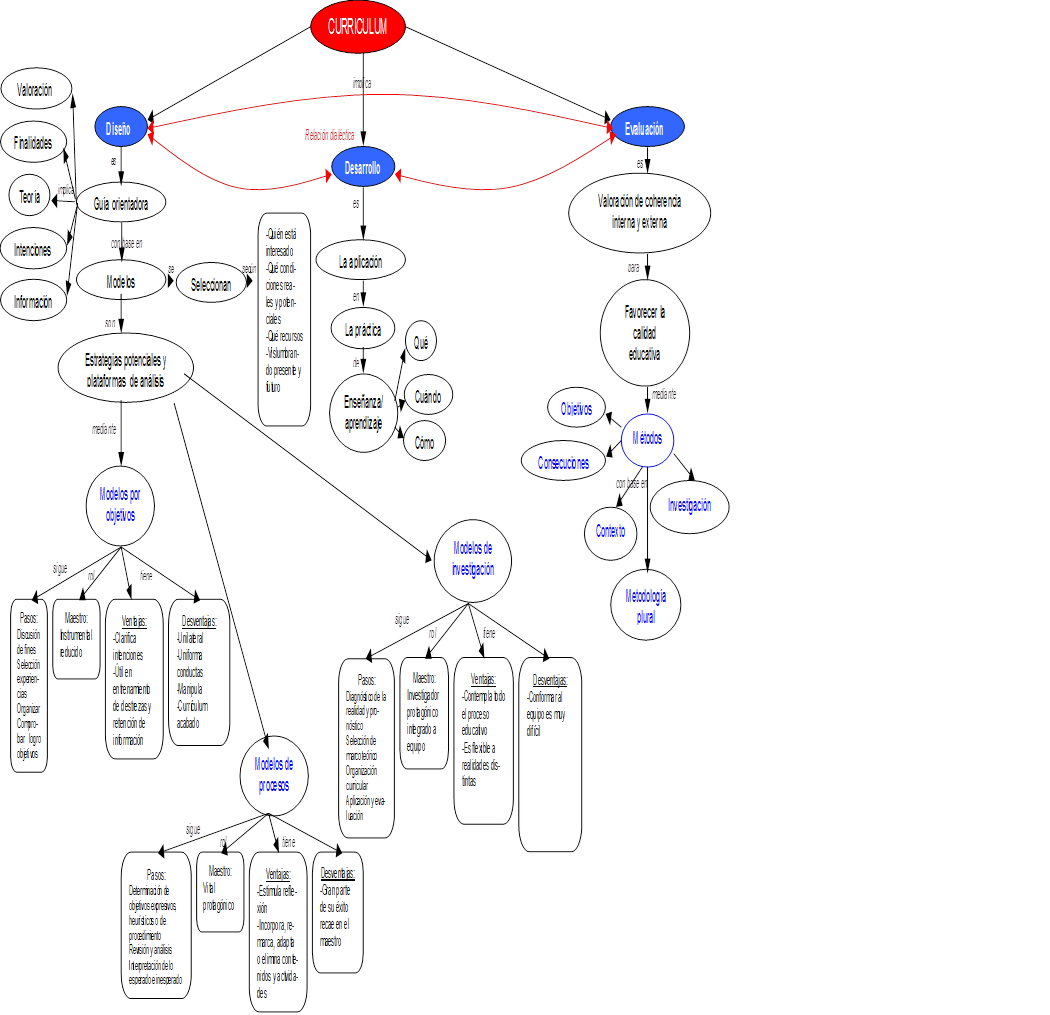
\includegraphics[width=16cm,height=16cm]{p3-img001.png}}
\end{figure}

{\footnotesize {\bfseries Fuente:} elaboración propia con base en Casarini (1999) y 
Stenhouse (1998).}
\newpage

Como referentes me basé en el modelo educativo orientado a la persona y  el cognitivo, así como en el enfoque constructivista, ya que lo consideré 
adecuado debido a la diversidad social, cultural y de procedencia de nuestro 
alumnado. Asimismo, sopesé las ventajas y desventajas de cada modelo 
para, acorde con la realidad y las intenciones pedagógicas, focalizar 
los aspectos positivos. 

En cuanto al sustento teórico, revisé tanto teorías sobre diseño 
curricular como sobre pedagogía, con la intención de que las y los 
alumnos que cursen esta Línea Terminal cuenten con conocimientos y 
herramientas que les permitan darle un giro mucho más dinámico, reflexivo 
y motivador a la enseñanza de la historia, sin descuidar el 
cumplimiento de los contenidos que estipulan los programas educativos 
del nivel en el que probablemente se desempeñen. 

Cabe señalar que el diseño inicial de la Línea Terminal fue discutido por la 
Comisión de reestructuración, integrada por cinco colegas. En este diseño curricular 
pusimos especial énfasis en la importancia de clasificar los objetivos tanto del Plan como 
del Programa de estudios. 

\enlargethispage{-1\baselineskip}
Como resultado del proceso, el actual Plan de estudios de  la 
Licenciatura en Historia de la UAQ, que se comenzó a implementar en 
agosto del 2010, tiene tres líneas terminales: Investigación, 
Patrimonio Histórico Cultural y Enseñanza de la Historia. La demanda 
para cada línea la conocemos al final del quinto semestre, que cuando el 
que el alumno decide. Cabe señalar que se ha documentado que el 
currículum oculto de las licenciaturas de Historia, en general, 
privilegia la investigación histórica sobre otras tareas propias del 
historiador (Rivera~2012). Díaz Barriga (2003,~p.~7) señala que el 
concepto de currículo oculto de \mbox{Jackson~(1968)}:
\newpage

\begin{quotation}
Restablecía la perspectiva que hemos denominado de 
la experiencia, articulando una serie de aprendizajes no explícitos en 
un plan de estudio, que no son intencionados, pero que se muestran 
altamente eficaces. Estos aprendizajes son resultado de la interacción 
escolar y en el aula; en este sentido, son resultados de la 
experiencia. 
\end{quotation}

Para Casarini (1999,~p.~42), <<El currículo se convierte en el mediador 
entre la escuela y la sociedad para lograr transmitir las intenciones 
educativas de una sociedad en determinado momento>>. 

Nuestro actual Programa de estudios busca que las y los alumnos 
desarrollen un papel activo y de responsabilidad frente al proceso 
educativo, por lo que toma como referente el enfoque constructivista, el 
cual propone que el conocimiento es parte integral de la actividad en la 
que se le adquiere,  y es significativo cuando ocurre en contextos 
relevantes y auténticos. Para esto, una de las características 
esenciales del diseño general de la licenciatura que nos ocupa es que 
el alumnado pueda cursar una materia genérica de cada una de las líneas 
terminales, ya sea en cuarto o quinto semestre, a fin de que su 
elección pueda tener elementos sustentados. La materia genérica o 
panorámica (obligatoria para quinto semestre) de la Línea Terminal que 
estamos abordando se denomina Enseñanza de la Historia, en ésta las y 
los alumnos adquieren los elementos necesarios para problematizar la 
práctica de la enseñanza de la Historia en diferentes ámbitos y 
contextos, cuestionar prácticas tradicionales de este quehacer a partir 
del análisis de modelos educativos, así como la revisión de su propia 
vida académica. Así, las y los estudiantes construyen elementos de 
decisión para ponderar si la Línea Terminal en Enseñanza de la Historia 
es su opción de especialidad (Latapí~2012).  
\newpage

%\enlargethispage{1\baselineskip}
El objetivo de la Línea Terminal en Enseñanza de la Historia 
enuncia que

\begin{quotation}
El egresado de la Licenciatura en Historia que haya cursado la Línea 
Terminal en Enseñanza de la Historia, tendrá las herramientas teóricas 
y metodológicas necesarias para participar en diversos ámbitos 
educativos: trabajo frente a grupo, servicios educativos en museos y 
elaboración de materiales educativos, entre otros. Podrá realizar su 
labor profesional con fundamento en el conocimiento del contexto en el 
que incidirá (UAQ 2010, p. 36).
\end{quotation}

Del sexto al octavo semestre, el alumnado de la Línea Terminal en 
Enseñanza de la Historia cursa seminarios, talleres y tópicos selectos 
especializados. <<Para la gradación, secuencia y tipo de asignaturas a 
ofrecer consideramos sustancial que el planteamiento de vinculación 
disciplinar estuviera al día en los paradigmas de la epistemología de 
las ciencias sociales, las psicopedagogías y la disciplina de la 
Historia>> (Latapí~2012,~p.~108). De esta manera, tuve presentes los niveles de 
Jantsch, retomados por Torres Santomé~(2000), y definidos sintéticamente 
de la siguiente manera: multidisciplinariedad como coordinación en el 
nivel más bajo, pero con comunicación incipiente; pluridisciplinariedad 
como intercambio de informaciones en un nivel de igualdad  jerárquica, 
con la virtud de que se unifican conocimientos de diferentes 
disciplinas, pero bajo la consigna de que se mantenga lo específico de 
cada una; disciplinariedad cruzada en la que una de las disciplinas 
domina sobre las otras, interdisciplinariedad que rebasa el reunir 
disciplinas en una marco u objetivo amplio, pues implica 
intercomunicación, trasformación  conceptual y metodológica con un 
equilibrio de fuerzas encaminadas a detectar y solucionar problemas de 
manera compleja; y transdisciplinariedad como la integración de alto 
nivel que posibilita la aparición de una metadisciplina.
\newpage

En lo que respecta al diseño de la  Línea Terminal en Enseñanza de la 
Historia en la UAQ, me enfoqué a rebasar los tres primeros niveles y a 
situar el Plan y Programa en el cuarto. La base sobre la cual 
construirlos parte de la idea de que de primero a quinto semestre los 
alumnos cursaron las asignaturas del eje formativo básico por medio del 
cual adquieren los conocimientos fundamentales de Historia, 
considerando los procesos históricos de larga duración de Europa, 
América, Asía y África, México y, finalmente, Querétaro y su región, 
desde una perspectiva que pretende no ser eurocéntrica. En cuanto al 
tiempo, se abarca desde los grupos prehispánicos, tanto de Mesoamérica y 
la región Andina, como de las primeras culturas clásicas, hasta el 
siglo XX\@. Se inicia en primer semestre con una materia que remite al 
mundo actual, de modo  que los alumnos establezcan relaciones del pasado con 
el presente.  También ya cursaron el eje formativo disciplinar, cuyo 
objetivo es dotarlos de herramientas teóricas y metodológicas 
necesarias para aprender el oficio de historiar, en las que llevan 
asignaturas relativas a las historiografías, a la escritura de la 
historia, a la teoría de la historia,  la historia oral y la 
paleografía, entre otras.  

\enlargethispage{1\baselineskip}
El diseño de los contenidos mínimos de los seminarios, talleres y 
asignaturas buscó la interrelación en el nivel de 
interdisciplinariedad. Espitia~(2002,~p.~16), señala que <<Entendemos la 
interdisciplinariedad como sinónimo de unión de las diferentes áreas en 
las que, de manera tradicional, se ha dividido el conocimiento>>.  
Asimismo, este autor agrega que
\begin{quotation}
La academia había hecho una división arbitraria, aunque no por ello 
ilógica de los contenidos de las materias. Dicha división responde más 
a las necesidades de transmisión que a la lógica del desarrollo de las 
disciplinas. Por esta razón, se hizo necesario pensar incluso los 
contenidos desde otra perspectiva. \ Al mismo tiempo los epistemólogos 
ponían \ en cuestión la excesiva especialización de la ciencia en la 
\mbox{actualidad}. Ambas cuestiones, la de la educación y la de la 
epistemología, aterrizan en el mismo lugar: \ la búsqueda de una 
concepción interdisciplinaria \ de los fenómenos. La 
interdisciplinariedad es solidaria con el pasaje de un pensamiento 
eminentemente racionalista a otro más complejo (\textit{ibid.}, p. 27).
\end{quotation}
%\newpage


Partiendo de la necesidad  que subyace en lo reseñado arriba, hoy entendemos 
que  la educación del siglo XXI debe tomar en cuenta
la cuestión de la interdisciplina como un aspecto medular, de tal forma que pueda encarar, explicar e intervenir en la complejidad de
la realidad social, y que deba plasmarse en todo el programa educativo (Latapí~2013). Por ello, antes de su implementación consideré que deberíamos estar conscientes de algunos puntos que se señalan enseguida: 

\enlargethispage{1\baselineskip}
Sabemos de sobra que en la <<aplicación>>  del Plan  y  Programa ---y que \ más \
que  ello será  una \ <<construcción>> \ en el vínculo entre docentes y alumnos--- un 
factor fundamental es el mediador que pueda enlazar y hacer 
significativos los saberes.  Así, pues, para nosotros, tanto al realizar 
el diseño curricular de la licenciatura y de las líneas terminales, 
como en la selección del personal docente para su implementación, hemos 
contemplado esta visión interdisciplinar, incluyendo a profesoras y 
profesores provenientes de diversas áreas de las ciencias sociales 
(psicología, antropología, educación,  comunicación, especialistas 
en equidad e igualdad de género, entre otros), buscando con ello llevar 
al alumnado a situarse en el lugar de protagonista del análisis e 
investigación del pasado, de sus herencias y memorias legadas a través 
del patrimonio, y de su enseñanza, de tal forma que pueda generarse en 
las futuras generaciones de estudiantes, ese gusto y comprensión por el 
estudio y el aprendizaje de la Historia, utilizándola como una asignatura 
que le permita la reflexión y el análisis del pasado, de una forma ágil y 
constructiva, de tal suerte que consiga aprender de ese pasado, y pueda 
mejorar el presente y el futuro de la sociedad a la que pertenece y el de 
su país. Así, entonces, con las 
diversas miradas sobre la realidad con que este profesorado media en nuestros 
estudiantes  y la complejidad de la interacción de la historia con 
otras ciencias sociales, también se presenta un balance cuando se integra con 
las miradas de los docentes que son historiadores (Latapí~2013). 

\enlargethispage{1\baselineskip}
Los contenidos mínimos de las asignaturas de  la  Línea Terminal en Enseñanza de la Historia, están engarzados entre sí. Enseguida doy cuenta de éstos. 
\begin{Obs} 
\item[$\star$] En sexto semestre los alumnos cursan dos 
seminarios, un taller y una asignatura de tópicos selectos. En el 
\textit{Seminario de Problemas de la Historia: perspectiva 
psicopedagógica\/} los alumnos,  con base inicial en lo abordado en 
otras asignaturas sobre todo del eje formativo disciplinario (La 
disciplina de la Historia y Enseñanza de la Historia de manera directa), 
deben identificar y conocer los principales problemas vinculados con la 
enseñanza de la Historia y que son derivados del carácter propio de los 
constructos de la disciplina, y analizarlos a la luz de los aportes de 
la psicología del desarrollo. También deben investigar un problema específico 
elegido a partir de sus intereses, y lo relacionarlo con un nivel 
educativo, para de ahí plantear posibles soluciones pedagógicas. La 
definición inicial de los problemas parte de los estudios realizados por 
Andrea Sánchez Quintanar, entre los que se encuentran los relativos 
al tiempo y espacio históricos, la causalidad, los sujetos de la historia. En el 
\textit{Seminario Ámbitos en la enseñanza de la Historia/} los alumnos 
analizan los diferentes ámbitos en los que se desarrolla la enseñanza 
de la historia: familia, escuela, medios de comunicación, Internet, 
barrios, museos, iglesias, ámbitos laborales y <<no lugares>>. 
Obedeciendo a sus intereses, elegirán un ámbito, e investigarán sus 
características económicas, sociales, políticas, culturales e 
ideológicas, a fin de identificar implicaciones concretas para la enseñanza 
de la historia. Los alumnos relacionarán dichos resultados de la
investigación con el problema vinculado a la enseñanza de la historia 
que trabajen en el {\itshape Seminario de Enseñanza de la Historia 1\/}, de tal
suerte que las soluciones pedagógicas planteadas sean adecuadas al contexto.  
En el \textit{Taller de Recursos Didácticos 1\/} los alumnos analizan 
críticamente diversos recursos educativos para la enseñanza de la 
historia (contenidos en programas, libros de texto, de divulgación y 
páginas web, entre otros) y diseñan uno de manera sustentada. La 
asignatura de \textit{tópicos selectos\/} es una materia cuyo contenido 
se establece de acuerdo con los intereses concretos de los alumnos.
\item[$\star$] En séptimo semestre las y los estudiantes cursan el 
\textit{Seminario de Praxis Docente\/}, en el que, con base inicial en lo 
abordado en los Seminarios de investigación 1 y 2, desarrollan un 
trabajo en el que deben articular la pertinencia teórica, el contexto y 
el ámbito elegido a la praxis docente. Los alumnos deben conocer  y 
tomar postura frente a los factores que inciden en una buena praxis 
docente. Aquí interviene la mediación de un proceso personal que no se 
ha mencionado y que es la propia experiencia de vida con respecto a 
docentes que han formado a los propios alumnos para hacer un ejercicio 
de toma consciencia, por ser este un factor que incidirá de manera 
directa en la praxis del alumno cuando sea docente. En el 
\textit{Seminario de Integración de problemas, ámbitos y praxis 
docente\/}, los  alumnos,  con base inicial en lo abordado en los 
Seminarios de Investigación 1 y 2, desarrollan un trabajo en el que 
articulan la pertinencia teórica, el contexto y el ámbito elegido que 
sustente su trabajo de titulación. En el {\itshape Taller de Recursos 
Didácticos II\/} \ los alumnos, apoyándose en el diseño del recurso 
didáctico que realizaron al principio en el {\itshape Taller de Recursos 
Didácticos~1\/}, desarrollan dicho recurso (con pertinencia pedagógica y 
disciplinar), lo finalizarán, lo aplicarán y lo evaluarán. Para ello podrán
valerse de las herramientas obtenidas en otras asignaturas, 
principalmente la de {\itshape Tecnología aplicada a la divulgación de la historia 1\/} y 
{\itshape 2}\@. 
\end{Obs}

\enlargethispage{1\baselineskip}
Siguiendo con la manera en que se ha buscado implementar una mirada 
interdisciplinaria, en la Licenciatura en Historia hemos fomentado que 
los estudiantes de la Línea Terminal en Enseñanza de la Historia, 
comprendan la necesidad de usar las fuentes del conocimiento histórico 
(investigación histórica) y del patrimonio cultural, tanto para 
sustentar argumentos como para ofrecer a los alumnos con quienes 
interactúan en sus prácticas profesionales, herramientas que les 
permitan problematizar la realidad histórica a través de procesos de 
enseñanza-aprendizaje, que les lleven a unir las asignaturas que cursan 
---que a sus ojos aparecen fragmentadas--- (historia, formación cívica, 
ética, geografía). En dichas asignaturas emergen algunas temáticas, como el 
cuidado del medio ambiente, la preservación, protección y conservación 
del patrimonio histórico cultural (en sus diferentes vertientes), los 
derechos humanos, entre otras, que sólo pueden ser abordadas desde la 
interdisciplina si se quiere lograr que dichos alumnos (adolescentes, 
principalmente) comprendan que las asignaturas son, precisamente, 
miradas sobre la realidad social que si las ponemos en tensión 
cognitiva y emocional, nos permiten asirla para comprenderla.

%\enlargethispage{1\baselineskip}
Así también, en la Línea Terminal en Enseñanza de la Historia, 
consideramos que las didácticas de la historia son de suma importancia para que 
los futuros docentes orienten a sus alumnos hacia aquellas tareas que 
generen niveles de comprensión altos y creativos, a través de plantear 
problemas y generar dinámicas que conduzcan al estudiantado a realizar 
preguntas al objeto o fenómeno, en búsqueda de la información histórica 
necesaria, y  hacia la reflexión teórica, partiendo de la relación que 
tenga la información recabada con los conocimientos, así como de la comunicación que 
sostenga con sus compañeros, sus profesores, especialistas en la materia y otros 
sujetos implicados en el proceso (Ferreiro,~López,~López, y~López~ 2004). 
El segundo referente que consideramos que deben tener nuestros 
estudiantes de las tres líneas terminales, es la búsqueda de la 
explicación histórica mediante la multidisciplinariedad, cuestión que 
reforzamos con los perfiles de nuestros docentes, quienes, como ya se 
mencionó, proceden de diversos campos de las ciencias sociales, con 
experiencias profesionales diversas. 

En cuanto a la aplicación de la perspectiva interdisciplinar en la 
Línea Terminal de Patrimonio, consideramos que éste, al ser 
un testimonio de toda una época, sirva, a través de objetos y 
manifestaciones relacionadas con la vida política, económica, social y 
espiritual de un lugar en un momento dado, como medio de 
enseñanza, y le permite al estudiante tener una visión más integral del 
contenido del aprendizaje. 

En cuanto a los alumnos que cursan la Línea Terminal en Investigación 
Histórica, se les fomenta la comprensión de la relación e incidencia 
que su trabajo tendrá a la hora de enriquecer el de sus compañeros que 
cursan las otras líneas terminales, así como lo fundamental que 
resulta nutrir su propio aprendizaje y el futuro desempeño profesional  
mediante la utilización de herramientas y conocimientos propios de 
disciplinas diversas, sin dejar de lado que, muy posiblemente, en su 
vida laboral enfrentarán situaciones que tendrán que ver con el 
patrimonio y la enseñanza en sus diversos ámbitos (enseñar siendo 
profesores universitarios, enseñar en un museo, enseñar en una 
publicación de cualquier índole, \ldots). 

%\enlargethispage{1\baselineskip}
Bajo tal supuesto se instrumentó  la materia de {\itshape Museos\/}, en la cual los alumnos deben desarrollar investigaciones y valerse de lo
aprendido sobre patrimonio para lograr generar, dentro de los museos, un espacio para enseñar historia.  Como
coordinadora de la Línea Terminal en Enseñanza de la Historia, he participado como invitada  en dicha asignatura,
experiencia que constituye un proceso colaborativo y que abre espacios para patentizar un currículum flexible.
%\newpage 

\medskip
\textbf{Resultados}

En el proceso de ponderar los diversos aspectos en vías a realizar modificaciones al Plan y Programa de estudios en el
2015, hemos diseñado y aplicado cuestionarios de evaluación a docentes y estudiantes, que ponen atención en la planeación de clases, la autorreflexión, el proceso de enseñanza-aprendizaje, la percepción global y particular de la Línea Terminal en Enseñanza de la Historia, así como en las prácticas profesionales y de servicio social. El análisis de estos cuestionarios nos arroja lo siguiente:
%\newpage

\bigskip
\begin{center}
\begin{tiny}       % otherwise, table won't fit
%\begin{table*}[h]
\tabulinesep=1.5mm
\begin{longtabu*} to \textwidth {X[5,l,p]|X[5,l,p]}
    %{X[50,l,l] | X[50,l,l]}
    %\caption[{}]\label{tab:label}\\ %
    \toprule
    %\hline \hline
\rowcolor{lsLightBlue}\textbf{DOCENTES} & \textbf{ALUMNADO}\\ 
    \midrule
  \endfirsthead%
%\hline \hline \hline \hline
%\begin{flushleft}
%\begin{table}[H]
%\begin{center}
%\begin{tiny}  % otherwise, table won't fit
%\tablefirsthead{%
%\hline
%{\bf DOCENTES} & {\bf ALUMNADO}\\
%\hline}
%\tablehead{}
%\tabletail{}
%\tablelasttail{}
%\bottomcaption{Figura 1. }
%\tablehead{\hline
%{\bf DOCENTES}  &
%\arraybslash{\bf ALUMNADO} \\\hline}
%\begin{supertabular}{|p{0.5\linewidth}|p{0.5\linewidth}|}
%\hline
%{\bf DOCENTES} & {\bf ALUMNADO}\\ 
%\hline
%\begin{center}
%\begin{landscape}
%\small  % otherwise, table won't fit
%\setlength\LTleft{-30pt}            % default: \fill
%\setlength\LTright{-30pt}           % default: \fill
%\begin{longtable}{|p{80mm}|p{80mm}|}
%\hline\hline 
%\multicolumn{1}{|l|}
%\footnotesize  % otherwise, table won't fit
%\setlength\LTleft{-30pt}            % default: \fill
%\setlength\LTright{-30pt}           % default: \fill
%\begin{longtable}{@{\extracolsep{\fill}}ll@{}}
%\hline\hline %inserts double horizontal lines
%{\bf DOCENTES} & 
%\multicolumn{1}{l|}
%{\bf ALUMNADO} \\ [0.5ex] \hline
%\endfirsthead 
%\multicolumn{2}{l}%
%{{\bfseries \tablename\ \thetable{} -- continuación}} \\
%Continuación de la tabla \\
%\hline 
%\multicolumn{1}{|l|}{
%{\bf DOCENTES} &
%\multicolumn{1}{l|}{
%{\bf ALUMNADO} \\ [0.5ex]  \hline 
%\endhead
%\hline \multicolumn{2}{|r|}{{continuación}} \\ \hline
%\multicolumn{2}{|r|}{{Continúa en la siguiente página}} \\
%\hline
%{ } & continúa... \\\hline \begin{tiny}
%\endfoot
%\hline
%{\bf DOCENTES} & 
%\multicolumn{1}{l|}{
%{\bf ALUMNADO} 
%\hline \hline
%\endlastfoot
%\endlastfoot
%\caption[(Cont)]
\multicolumn{2}{r}{{Viene de la página anterior\ldots}} \\ \midrule %\hline
%{\emph{Continuación}}\\%
\toprule
\rowcolor{lsLightBlue}\textbf{DOCENTES} & \textbf{ALUMNADO}\\ 
\midrule
\endhead%
\bottomrule
\multicolumn{2}{r}{{Continúa en la siguiente página\ldots}} %\\\ %hline
\endfoot%
%
%\hline
\midrule\endlastfoot%
% Now the regular content:
\rowcolor{lsLightGray} \textbf{Autorreflexión} 

Interés docente por compartir conocimientos y experiencia profesional 
en diferentes ámbitos con las y los alumnos, con la intención de 
incidir positivamente en la mejora en la enseñanza de la historia por 
considerarla vital para educar a los seres humanos en la comprensión, 
la empatía y el humanismo, desarrollando en ellos una visión que les 
permita conocer sus orígenes, quienes son y cómo pueden enriquecer su 
presente. 

La mayoría de las y los docentes hicieron recomendaciones al alumnado
para mejorar la redacción y ortografía, exposición en clase, aprendizaje, 
presentación de trabajos y actitud en clase. 
&

{\bfseries Autorreflexión}

Interés del alumnado por aportar a las futuras generaciones una visión
diferente de la historia, su aprendizaje y su enseñanza.

Las y los alumnos consideran que escucharon y pusieron en práctica
todas las sugerencias de mejora y recomendaciones que les hicieron las y los 
docentes.\\
%\midrule
\addlinespace
\rowcolor{lsLightGray} {\bf Planeación de clases}

Las y los docentes entregan un programa del curso y lo comentan con el
alumnado, aclarando dudas, técnicas de enseñanza, fuentes de información y formas 
de evaluación. 

La mayoría piensa que la secuencia, orden y relación de presentación y
trabajo de los temas que se ven en clase permiten al alumnado lograr un aprendizaje significativo. 

Algunos docentes consideraron que un área de mejora es la comunicación
entre docentes para conocer los contenidos de sus asignaturas, áreas de oportunidad del alumnado y 
cargas de trabajo asignadas a las y los alumnos. 
&
{\bfseries Planeación de clases}

Las y los alumnos coinciden con la respuesta de las y los docentes en
cuanto a la entrega y discusión del programa del curso.  

La respuesta del alumnado coincide con la de las y los docentes.\\
%\hline
\addlinespace 
 
\rowcolor{lsLightGray} {\bfseries Proceso enseñanza–aprendizaje}

La mayoría de las y los docentes:

\begin{itemize}
\item Utilizan como materiales la Antología que entregan al inicio del
curso, libros, diagramas, esquemas y mapas conceptuales. 
\item  Relacionan la teoría con ejemplos y\slash\o situaciones
prácticas.
\item  Las principales fuentes y medios que promueven para la consulta
de información son: la biblioteca, Internet, revistas y libros. 
\item Brindaron asesoría al alumnado.
\item Consideraron que el ambiente de trabajo en clase fue bueno o
regular.
\item  Consideran que las asignaturas de la Línea Terminal, así como las
de ésta con las de las de otras de la licenciatura y Líneas Terminales, se relacionan mucho entre sí. 
\item Coinciden en evaluar la actitud para el aprendizaje de las y los
alumnos entre buena y regular. 
\item  Utilizan como forma de evaluación los exámenes y trabajos
escritos, trabajo e investigación de campo, exposición en clase y tareas. 
\item  Durante el desarrollo del curso fomentan la discusión en clase,
la crítica razonada, el auto aprendizaje, el razonamiento científico, el trabajo en equipo De los 7 docentes solamente
3 fomentaron la utilización de la perspectiva de género en el desarrollo del curso (2 de ellas ya no colaboran con
nosotros).
\item  Encontraron que las y los alumnos solamente a veces y en algunos
casos, revisan y ponen en práctica las sugerencias de mejora o correcciones hechas a sus trabajos.
\end{itemize}
&
{\bf Proceso enseñanza-aprendizaje}

La mayoría de las y los alumnos: 

\begin{itemize}
\item  Utilizan y les son de mayor utilidad los materiales como:
antología, libros de texto, vídeo, ejercicios prácticos, diagramas, esquemas y mapas conceptuales. 
\item Coinciden en que las asignaturas que relaciona más la teoría con
la práctica son Taller de Recursos Didácticos I y II\@. 
\item Consideran que la dinámica principal de las clases son
expositivas, con participación de ellas y ellos. 
\item  Opinan que las principales fuentes y medios que las y los
docentes promovieron para la consulta de información fueron: Antologías de textos, páginas de Internet y libros.
\item Dijeron que las y los docentes les brindaron apoyo o asesoría
cuando se les solicitó. Opinaron que el nivel de calidad y apoyo brindado fue bueno (en un rango de excelente a malo).
\item  Consideraron que el ambiente de trabajo promovido por las y los
docentes fue bueno (en un rango de excelente a malo).
\item  Consideraron en promedio como <<bueno>> el nivel de conocimiento de
la asignatura por parte de las y los docentes (en un rango de excelente a malo). En este punto hubo contradicciones
pues hay calificaciones de excelente, malo y regular para un mismo docente. 
\item  Opinan que las asignaturas de la LT se relacionan <<más o menos>>
con otras de la licenciatura o de las otras LT\@. 
\item  Consideran que en las formas o criterios de evaluación predomina
el trabajo escrito, el proyecto y las tareas. 
\item  Consideran que dos docentes promueven la discusión en clase, la
crítica razonada, el autoaprendizaje, la perspectiva de género, el razonamiento científico, el trabajo en equipo. Tres
docentes promueven los trabajos de investigación y el análisis de la relación de lo sucedido a nivel internacional en
una misma época con el presente.
\item  Consideran que la mayoría de las y los docentes dieron
retroalimentación a sus trabajos y tareas. 
\item Consideran que los contenidos de la LT son actuales, relevantes
para su formación y comprensibles. 
\end{itemize}

Las respuestas en cuanto a las y los profesores que impulsan o no la
participación en clase para mejorar el aprendizaje fueron variadas y 
contradictorias.\\
%\hline
\addlinespace
 
\rowcolor{lsLightGray} {\bfseries Percepción global}

La mayoría de las y los docentes:

\begin{itemize}
\item  Evaluaron bajo la actuación conforme a valores de parte del
alumnado, así como la actitud hacia el aprendizaje y el compañerismo. 
\end{itemize}
&
{\bf Percepción global}

La mayoría de las y los alumnos:

\begin{itemize}
\item  Evaluaron alto a las y los docentes en cuanto a la promoción de
valores en su praxis docente. 
\end{itemize} \\
%\midrule
\addlinespace 

\rowcolor{lsLightGray} {\bfseries Percepción Línea Terminal}

La mayoría de las y los docentes consideraron que:

\begin{itemize}
\item  Los mejores aspectos de la Línea Terminal son la relación de los temas
entre las asignaturas, el programa de estudios, las prácticas profesionales, los eventos (congresos, seminarios, etc.) que fortalecen el aprendizaje y el servicio social. 

\item Las fortalezas de la Línea Terminal (LT) son: el entusiasmo de las y
los docentes; el eje formativo permite al alumnado aplicar y relacionar los conocimientos previos; impulsa una
formación integral que afianza a las materias con las actividades fuera del aula; formar historiadores como enseñantes,
con estrategias didácticas y fundamentos pedagógicos.

\item Las debilidades de la Línea Terminal son: al inicio del semestre 
el alumnado se enfrenta con temas y dinámicas nuevas; las y los alumnos 
se sienten menos que los que cursan otras LT\@; relacionar los contenidos 
de las asignaturas y especialmente los trabajos y proyectos de forma 
horizontal, promover la colaboración y comunicación entre el 
profesorado; fortalecer la exposición en clase por parte del alumnado, 
así como la utilización de la perspectiva de género, tanto en la praxis 
docente como en la investigación y enseñanza de la historia.

\item  Las áreas de oportunidad de la Línea Terminal son: fortalecer el
trabajo colectivo docente así como las habilidades de investigación, aun cuando la especialidad sea en enseñanza; mejorar el compromiso de las y los alumnos.

\item El alumnado debe fortalecer la capacidad de análisis y abstracción,
síntesis, redacción, metodología de investigación, utilización de las TIC, idioma inglés.

\item Considera que las asignaturas de la LT son de utilizad para el
desempeño del alumnado en diferentes ámbitos en la enseñanza de la historia. 
\end{itemize}
&
{\bf Percepción Línea Terminal}

La mayoría de las y los alumnos consideraron que: 

\begin{itemize}
\item Los aspectos que más les han gustado de la LT son: las prácticas
profesionales, el servicio social y los eventos. 
\item Las asignaturas cursadas en la LT les son de utilidad para
desempeñarse en diferentes ámbitos en la enseñanza de la historia.
\item  La cantidad de lecturas y trabajos por semestre fueron apropiados
para su aprovechamiento académico. 
\end{itemize} \\
%\midrule
\addlinespace 
 
\rowcolor{lsLightGray} {\bf Servicio social y prácticas profesionales}

Algunos docentes consideran que los lugares en donde las y los alumnos
realizan su servicio social y prácticas profesionales son los adecuados pues pueden practicar la docencia. 
&
{\bf Servicio social y prácticas profesionales}

La mayoría de las y los alumnos considera que:

\begin{itemize}
\item El servicio social contribuye a su consolidación académica.
\item Las prácticas profesionales que realizaron contribuyen a su
formación para la enseñanza de la historia. 
\end{itemize} \\
%\hline
\addlinespace
\bottomrule
\end{longtabu*}

%\end{supertabular}
%\end{longtable}
%\end{table}
%\end{flushleft}
%\caption*{Cuadro 1}
%\end{footnotesize}\end{center}
%\end{table*}
%\end{center}
\end{tiny}\end{center}
\normalsize
\newpage

Actualmente, la primera generación de la Línea Terminal en Enseñanza de la Historia está finalizando sus estudios y, aun cuando a lo largo del camino hubieron encuentros y 
desencuentros entre el alumnado y las y los docentes, la línea está bien valorada, como se puede
colegir de las evaluaciones en cuanto al ambiente de trabajo, así como en las del 
profesorado en cuanto a actuación conforme a valores, actitudes frente al aprendizaje, compañerismo y puesta en práctica de la retroalimentación. Con
base en ello podemos decir que, a mitad de camino, tenemos tanto resultados positivos 
y prácticas para volver a implementar,  como áreas de posible mejora. 

Desde el punto de vista tanto de las y los docentes como del alumnado, las siguientes son las fortalezas de esta línea terminal: considerar que las asignaturas cursadas 
en ella son de utilidad para que el alumnado se desempeñe 
en diferentes ámbitos en la enseñanza de la historia; el gusto y la
pertinencia de la realización y la asistencia a eventos; la repercusión de las 
prácticas profesionales y el servicio social, pues le permite al alumnado poner en 
práctica las estrategias y teorías aprendidas en la especialidad. Un 
aspecto  que demanda especial atención es la diferencia en la percepción entre 
alumnado y el profesorado sobre la relación que se da entre las asignaturas cursadas 
en la Línea Terminal en Enseñanza de la Historia con otras de la licenciatura 
o de otras Líneas Terminales. 

\enlargethispage{1\baselineskip}
Como debilidades encontramos la necesidad de fortalecer la investigación y la exposición en clase por parte del alumnado,
así como el fomento de la discusión en clase y la crítica razonada, así como la utilización de la perspectiva de
género, tanto en la praxis docente como en la investigación y enseñanza de la historia. Asimismo, es importante crear
una biblioteca con materiales específicos para las y los estudiantes de nuestra Línea Terminal.

Las áreas de oportunidad que detectamos se refieren, básicamente, a la necesidad de fortalecer el trabajo en colectivo de las y los docentes, así la capacidad de análisis y abstracción, síntesis, redacción, metodología de la investigación, utilización de las TIC y de materiales en inglés por parte de las y los alumnos. 

\bigskip
\noindent {\bfseries Referencias}
\enlargethispage{1\baselineskip}

\medskip
Casarini, M\@. (1999), \textit{Teoría y diseño curricular}, México, Ed\@. Trillas-UV\@. 

Díaz Barriga, A. (2003), <<Currículum. Tensiones conceptuales y prácticas>>. En 
\textit{Revista Electrónica de Investigación Educativa, 5}. Consultado el 3 de marzo de 2011 en \\
\url{http://redie.uabc.mx/vol5no2/contenido-diazbarriga.html}

\begin{sloppypar}
Ferreiro, R., López, J., López, L. y López, J. (2004), <<El patrimonio cultural entre los medios de enseñanza de la Historia>>. \textit{Ilustrados, 1--4}. Recuperado el 12 de marzo del 2013 de \url{http://www.ilustrados.com/tema/7180/patrimonio-cultural-entre-medios-ensenanza-Historia.html}
\end{sloppypar}

Latapí, P. (2012), \textit{Construyendo sobre las miradas en torno a la enseñanza de 
la Historia}. En Latapí, P., Miró, M. y Somohano, L. (coords), \textit{Miradas diversas. Estudios Antropológicos, Históricos y Filosóficos},\\ pp.106--116. México, UAQ-Facultad de Filosofía.  

Latapí, P. (2013), La interdisciplinariedad en las Licenciaturas en Historia. En \textit{VIII Encuentro de la Red Nacional de Licenciaturas en Historia y  Cuerpos Académicos y $2^\circ$  Encuentro Iberoamericano de Licenciaturas}. En \textit{Historia. <<Currículo, formación y práctica docente en la enseñanza de la Historia>>}, Morelia, Michoacán, Facultad de Historia, Universidad Michoacana de San Nicolás de Hidalgo.

Luhmann, N. (1973), \textit{Ilustración sociológica y otros ensayos}, Buenos Aires, Sur.

Rivera Gómez, E. (2012), <<Investigación y enseñanza de la Historia: una reflexión desde la práctica académica>>. En Latapí, P., Miró, M. y Somohano, L. (coords). \textit{Miradas diversas. Estudios Antropológicos, Históricos y Filosóficos}, (pp. 18--24). México, UAQ-Facultad de Filosofía.  

Stenhouse, L. (1998), \textit{Investigación y desarrollo del currículum}, Madrid, Morata.

Torres Santomé, J. (2000),  \textit{Globalización e interdisciplinariedad: el currículum integrado}, Madrid, Morata.

\begin{sloppypar}
Wallerstein, I\@. (1996), \textit{Abrir las ciencias sociales}, México, Siglo XXI-Centro de Investigaciones Interdisciplinarias en Ciencias y Humanidades UNAM\@.
\end{sloppypar}

Wallerstein, I\@. (1999), \textit{Impensar las ciencias sociales}, México, Siglo XXI-Centro de Investigaciones Interdisciplinarias en Ciencias y Humanidades UNAM\@.

%\clearpage\setcounter{page}{65}
%\markboth{}{}
\thispagestyle{empty}	
\phantomsection{}
\addcontentsline{toc}{chapter}{La enseñanza de la Historia y su pertinencia\\ en los Planes de Estudio\newline $\diamond$
\normalfont\textit{María Gabriela Guerrero Hernández\\ y María del Rocío Rodríguez Román}}	
{\centering{\scshape \large La enseñanza de la Historia y su pertinencia\\ en los Planes de Estudio} \par}
\markboth{formación del historiador}{la enseñanza de la historia}

\bigskip
\begin{center}
{\bfseries  Ma. Gabriela Guerrero Hernández\\
María del Rocío Rodríguez Román}\\
{\itshape{} Facultad de Filosofía y Letras de la UANL\/}
\end{center}


\bigskip
\noindent{\bfseries Resumen}

La docencia y\slash{}o enseñanza de la historia es una de las 
acentuaciones o fases terminales presentes en las distintas 
Licenciaturas de Historia que se ofertan en México, situación que 
merece ser analizada para identificar qué criterios se han considerado 
al respecto para la denominación de las unidades de aprendizaje que 
conforman y, a la vez, amplían la formación de los futuros Licenciados 
en Historia, así como su contenido. Aspectos por demás importantes para 
comprender la relevancia que esta acentuación cobra en los últimos 
años, sobre todo a partir de las demandas del mundo globalizado que 
requiere de un profesionista con conocimientos actualizados y que estén 
acordes con las necesidades del mercado; lo que lleva a considerar que 
el egresado de Historia no sólo debe ser capaz de explicar los procesos 
socio-históricos por los que ha transitado la humanidad a través del 
tiempo, sino que también debe poseer los recursos didácticos  para 
acercar a las generaciones más jóvenes al conocimiento histórico.\\ 
{\bfseries Palabras clave:} Plan de Estudios, enseñanza de la historia, 
procesos formativos, especialización y malla curricular.
%\enlargethispage{\baselineskip}

\medskip
\textenglish{{\bfseries Abstract}}

\textenglish{History Teaching and its Relevance to the Curriculum 
Teaching of history is one of the accentuations or ending phases in all 
the different degrees in history offered in Mexico. This situation 
deserves to be analyzed to identify the criteria considered in the 
denomination of the learning units that are part, and at the same time 
expanded of the formation of future graduates with a bachelor's degree 
in history and its content. These aspects are vital to comprehend the 
relevancy of this accentuation in the last few years, specially because 
of the demand of our globalized world that requires a professional with 
date knowledge lined whit market needs. This reads us to considerate 
that the graduate whit a bachelors degree in History should not only be 
able to explain the process social-historical by which humanity has 
transited over time but should possess the teaching resources to bring 
the younger generations to the historic knowledge.}\\ 
\textenglish{\textbf{Keywords:} Curriculum, Teaching of History, 
Training Processes, Specialization.}

\medskip 
\noindent La enseñanza de la historia es una de las dos áreas  
principales del quehacer del historiador como bien lo ha señalado Plá 
(2011), no obstante, esta área es poco valorada incluso por los mismos 
historiadores, quienes durante su formación han sido receptores de un 
discurso que privilegia la investigación e interpretación de los hechos 
del pasado, en  menoscabo de la formación orientada hacia la enseñanza 
de la historia, situación que poco se ha llevado a la discusión, en 
parte porque la tradición sigue presente en los procesos formativos de 
los estudiantes de la licenciatura en historia, y, por otra parte, 
porque incluso ni los mismos formadores de esta disciplina han 
reflexionado que una de las bondades de la profesión es también el 
difundir el conocimiento histórico a través de su enseñanza, y que para 
ello se requiere ampliar los saberes presentes en el Plan de Estudios 
bajo el cual se prepara a los futuros licenciados en Historia.  

%\enlargethispage{1\baselineskip}
Cabe señalar que esta preocupación es relativamente reciente en el 
ámbito de la universidad, debido a que en esta institución se mantiene 
la tradición en relación a la promoción de la investigación, lo cual es 
positivo, pero siempre y cuando no se descuiden las otras dos funciones 
sustantivas de la universidad, como son la docencia y la difusión de la 
cultura. Como lo  ha expresado Fabre (2005, p. 6), quien encuentra que desde 
la Organización de las Naciones Unidas para la Educación, la Ciencia y 
la Cultura (UNESCO) se insiste en que las universidades del siglo XXI 
son <<Centros de ciencia y fuente de conocimiento que llevan a la 
investigación teórica o aplicada o a la formación de profesores>>, lo 
cual indica que la docencia y\slash{}o enseñanza de la historia debe 
tener un estatus similar al de la investigación.
 
Quizás esta sea una de las orientaciones que recientemente han permeado 
a la universidad pública, la cual ha entrado en una dinámica de cambio, 
producto de las transformaciones en los distintos campos de la 
sociedad (económico, político, social y cultural), que la han llevado a 
replantearse su papel en la formación de los futuros profesionistas y a 
incorporar las tendencias educativas más actuales en sus Planes y 
Programas de Estudio, como es el modelo educativo por competencias y el 
enfoque del aprendizaje centrado en el alumno.  Tendencias que se 
complementan y sugieren un cambio de paradigma educativo en la 
universidad, quien, atenta a estos cambios, se ha dispuesto a incorporar 
de manera gradual las recomendaciones mediante unos procesos de rediseño 
curricular, cuyo impacto se observa ya en la malla curricular con que se 
forman a los estudiantes; por lo menos es lo que se ha encontrado en la 
revisión que se ha llevado a cabo de los 39 Planes de Estudio ofertados 
en las universidades del país. 
\enlargethispage{-1\baselineskip}

El desarrollo de competencias didácticas en los programas educativos de 
Historia a nivel licenciatura debe ser una parte medular, pues es 
sabido que la docencia y  la investigación  son las actividades 
sustantivas de todo historiador: <<El historiador profesional 
universitario[\ldots] combina una dualidad de funciones bien conocida: es y 
debe ser investigador y enseñante al mismo tiempo>> (Moradiellos 
1994, p. 62). 

Pensar que la tarea del historiador consiste sólo en  crear nuevo 
conocimiento, es decir, en buscar los hechos, analizarlos e 
interpretarlos, es limitar demasiado su función. Por eso la enseñanza 
universitaria de la historia debe incluir tanto la parte disciplinar; 
es decir, el cuerpo de conocimientos de la historia,  como la parte 
práctica, o sea la formación sobre cómo se produce dicho conocimiento, 
y además el elemento didáctico, que hace referencia a cómo enseñar la 
historia. Ya que, como señala Andrea Sánchez Quintanar (1995, p. 3), 

\begin{quotation}
(\ldots) la formación como la información del futuro historiador se orienta 
mucho más hacia la investigación que hacia la docencia, pese a que por el 
contrario, el terreno de la práctica profesional es mucho más amplio en 
la enseñanza escolar. 
\end{quotation}

\enlargethispage{1\baselineskip}
Motivo por el cual resulta necesario conocer en qué medida los 
programas educativos de Historia que, a nivel licenciatura, ofrecen las 
diferentes universidades del país, tanto públicas como privadas, 
contemplan el desarrollo de competencias didácticas en sus estudiantes. 
De acuerdo al Catálogo de la Asociación Nacional de Universidades e 
Instituciones de Educación Superior (ANUIES) 2012,  existen en el país 
34 Instituciones de Educación Superior (IES) incorporadas a esta 
asociación, entre las cuales ofrecen 39 programas de Licenciatura en Historia 
o carreras afines (Ver Anexo 1).  Con base en la información proporcionada en 
las páginas electrónicas de las IES, se hizo una revisión de los 
perfiles de egreso, pues ahí es donde se indica el tipo de 
profesionista que se espera formar, con el propósito de identificar la 
idea que subyace en cada una de ellas respecto a lo que implica el 
oficio del historiador,  misma que se ve reflejada en la malla 
curricular que forma a los estudiantes como futuros historiadores.

De los 39 programas educativos no se localizó el perfil de egreso de 
nueve de ellos, y de los treinta restantes solo en siete no se hace 
ninguna alusión a la docencia, sino que son muy genéricos.  Los 23 
restantes sí señalan que se espera que al egresar los estudiantes se 
desarrollen en la investigación, la docencia, la difusión y\slash{}o 
preservación del patrimonio cultural,  como las áreas fundamentales del 
quehacer del historiador. Lo que indica que, al menos en el discurso, se 
considera que la función del historiador va más allá que la de investigar.

\enlargethispage{1\baselineskip}
Ahora bien, revisando las mallas curriculares se pudo observar lo 
siguiente: no hay proporción entre las unidades de aprendizaje (UA) 
relacionadas con la docencia, la investigación y la difusión, pues dos 
terceras partes se avocan a formar a los estudiantes en la 
investigación, un 21.9\,\% a la docencia y solo un 14.6\,\% a la 
difusión (véase el Cuadro 1). 

\begin{small}
\textbf{Cuadro 1. Unidades de aprendizaje relacionadas con las áreas de 
docencia, investigación, difusión o patrimonio en las mallas 
curriculares} 
\end{small}

\begin{flushleft}
%\tablefirsthead{}
%\tablehead{}
%\tabletail{}
\begin{supertabular}{m{1.7cm}m{1.7cm}m{1.7cm}m{1.7cm}m{1.7cm}m{1.7cm}}
\hline
\multicolumn{2}{>{\columncolor{sLightGreen}} m{3.6cm}}{\centering \bfseries DOCENCIA}&
\multicolumn{2}{>{\columncolor{sLightGreen}} m{3.6cm}}{\centering \bfseries INVESTIGACIÓN}&
\multicolumn{2}{>{\columncolor{sLightGreen}} m{3.6cm}}{\centering \bfseries DIFUSIÓN}\\[1pt]
%\hline

\rowcolor{sLightGreen}{\centering{\textbf{\phantom{ab}No.}}}&\centering{\textbf{\%}}&\centering{\textbf{No.}} 
&\centering{\textbf{\%}}&\centering{\textbf{No.}}&
\centering\arraybslash{\textbf{\%}}\\%\hline

\rowcolor{lsLightGray}\centering{\textbf{66}}&\centering{\textbf{21.9}}&\centering{\textbf{191}}&
\centering{\textbf{63.4}}&\centering{\textbf{44}}&\centering\arraybslash{\textbf{14.6}}\\\hline\hline

\multicolumn{6}{>{\columncolor{lsLightGray}} m{11.2cm}}{\textbf{\footnotesize Fuente:} {\footnotesize Mallas curriculares de las Licenciaturas de Historia incorporadas a la ANUIES.}}\\%\hline
\end{supertabular}
\end{flushleft}
%\newpage

Cabe aclarar que solo se consideraron las 
unidades de aprendizaje que aparecían como obligatorias en las mallas 
curriculares, pues cada programa educativo ofrece varias asignaturas 
optativas relacionadas con estas tres áreas terminales o acentuaciones. 

Respecto al número de UA, destaca el hecho que en seis de los 
39 programas revisados, no se ofrece ninguna materia obligatoria 
relacionada con la formación docente, y que en solo dos de estos programas 
se ofrecen unidades de este tipo,  pero como optativas, lo que significa que no es 
seguro que los estudiantes las elijan. Ahora bien, encontramos que en dos 
de estos programas sí se considera la docencia como parte de la 
formación de los futuros historiadores, aunque no se explica cómo 
lograran las competencias docentes si no cuentan con ninguna unidad de 
aprendizaje relacionada con ello; mientras que en otros tres programas 
están entre los que no se consiguió su perfil de egreso.

\enlargethispage{\baselineskip}
Llama la atención, en este sentido, el caso de la UANL, pues en su plan de estudios 
2005 todas las materias vinculadas con la docencia son de carácter optativo, lo que 
significa que si los jóvenes no eligen esa acentuación salen de su 
carrera sin ninguna base para hacer frente a la actividad docente. Como lo 
constatan las cifras: en las diez generaciones que han egresado hasta ahora, 
solo tres estudiantes han elegido dicha fase terminal. Hecho que fue tomado en 
cuenta a la hora de hacer el rediseño del Plan de estudios que fue aprobado el año 
pasado (2013), pues para evitar que esto siguiera sucediendo se eliminaron las 
acentuaciones y se establecieron como obligatorias tres unidades 
relacionadas con la formación didáctica.  

En 13 programas educativos solo se ofrece una UA que tiene que ver con 
la formación docente, lo que a todas luces resulta insuficiente para 
desarrollar competencias docentes en los estudiantes; mientras que 
solo en cinco de ellos se ofrecen UA optativas. Con dos UA se encontraron 
11  programas educativos, de los cuales solo dos tienen UA optativas, 
siendo también reducidas las opciones que tiene el estudiante a la hora de 
formarse para la actividad docente.  Dos programas ofrecen cuatro UA obligatorias 
relacionadas con la formación didáctica, y solo un programa ofrece 
cinco; aunque ninguno de ellos ofrece unidades optativas de esta 
índole, lo que revela que en estas carreras se considera que esa cantidad 
es suficiente para que el estudiante desarrolle las competencias didácticas 
requeridas para hacer frente a los retos que la enseñanza implica (véase el Cuadro 2). 

\bigskip
\begin{small}
\textbf{Cuadro 2. Cantidad de unidades de aprendizaje\\ relacionadas con 
el área de la docencia en las mallas\\ curriculares}

\medskip
\begin{flushleft}
\tablefirsthead{}
\tablehead{}
\tabletail{}
\tablelasttail{}
\begin{supertabular}{|m{2.2cm}m{1.0cm}m{1.0cm}m{1.0cm}m{1.0cm}m{1.0cm}m{1.0cm}m{1.73cm}|}
\hline%\hline
\rowcolor{sYellow}\centering{\textbf{U de A por PE}} &
\centering{\textbf{0}} &
\centering{\textbf{1}} &
\centering{\textbf{2}} &
\centering{\textbf{3}} &
\centering{\textbf{4}} &
\centering{\textbf{5}} &
\centering\arraybslash{\textbf{Totales}}\\\hline

\centering{No.} &
\centering{6} &
\centering{13} &
\centering{11} &
\centering{6} &
\centering{2} &
\centering{1} &
\centering\arraybslash{39}\\\hline

\centering{\%} &
\centering{15.3} &
\centering{33.3} &
\centering{28.2} &
\centering{15.3} &
\centering{5.1} &
\centering{2.5} &
\centering\arraybslash{100}\\\hline\hline
\multicolumn{8}{>{\columncolor{lsLightGray}} m{0.98\textwidth}}{\footnotesize\textbf{Fuente:} {\footnotesize Mallas curriculares de las Licenciaturas de Historia incorporadas a la ANUIES}}\\%\hline
\end{supertabular}
\end{flushleft}
\end{small}

\bigskip
\enlargethispage{\baselineskip}
Si esto se compara con las otras dos  acentuaciones, resulta 
significativo observar que 19 de los 39 programas no ofrecen 
unidades obligatorias vinculadas con la difusión, y solo en siete de 
éstos existe la variante de unidades optativas. Esto de alguna manera 
refleja que esta área formativa recién se está incorporando a los 
programas, quizás a raíz de que ha sido en los últimos años cuando se 
han incrementado las posibilidades de que los egresados se inserten en 
estos espacios laborales relacionados con la difusión y el cuidado del 
patrimonio histórico. 

En cuanto toca a la investigación, encontramos que en todos los programas 
educativos hay por lo menos una UA obligatoria relacionada con esta área; 
y que el máximo de UA de este tipo es diez. Incluso en algunos casos, en 8 
de los programas educativos analizados, para ser exactos, se tienen más 
opciones de formarse en esta área, dado que cuentan con unidades optativas
relacionadas. Este fenómeno no resulta extraño, pues es un hecho que 
la investigación sigue siendo el área más fuerte en la formación de 
los historiadores (véase el Cuadro~3).
%\newpage

\bigskip
\begin{scriptsize}
\textbf{Cuadro 3. Unidades de aprendizaje
relacionadas con las áreas de difusión\\ e investigación en las mallas  
curriculares}
\end{scriptsize}

\medskip
\begin{center}
\begin{scriptsize}
\tablefirsthead{}
\tablehead{}
\tabletail{}
\tablelasttail{}
\setlength{\extrarowheight}{1.5pt}
%\begin{tabular}{m{25mm}rcccccccccccr}
\begin{supertabular}{m{18mm}ccccccccccccr}
%{m{1.815cm}m{0.50cm}m{0.55cm}m{0.55cm}m{0.55cm}m{0.55cm}m{0.6cm}m{0.6cm}m{0.60cm}m{0.55cm}m{0.5cm}m{0.25cm}m{0.4cm}m{0.95cm}}
\hline%\hline

%\toprule[1.5pt]
%\rowcolor{lsLightBlue}\multicolumn{2}{m{2.8cm}}{\textbf{U de A por PE}} &
\rowcolor{white}\multicolumn{2}{m{24mm}}{\textbf{U de A por PE}}&
0 & 1 & 2 & 3 & 4 & 5 & 6 & 7 & 8 & 9 & 10 & \arraybslash{Total}\\\hline
\rowcolor{sLightGreen}\multirow{2}{*}{Difusión} & No. & 19 & 6 & 6 & 6 & 2 & 0 & 0 & 0 & 0 & 0 & 0 & 39 \\%\hline %\arraybslash{39}\\
%\hline
%\cline{2-13}
\rowcolor{sLightGreen} & {\scriptsize \%} &
48.7 &
15.3 &
15.3 &
15.3 &
5.1 &
0 &
0 &
0 &
0 &
0 &
0 & 
%\arraybslash{99.7} \\\hline
99.7 \\\hline
\rowcolor{sYellow}\multirow{2}{*}{Investigación } &
{\scriptsize No.} &
0 &
2 &
1 &
6 &
9 &
5 &
9 &
4 &
2 &
0 &
1 & 
%\arraybslash{39} \\\hline
39 \\%\hline
\cline{2-14}
\rowcolor{sYellow} & {\scriptsize \%} &
0 &
5.1 &
2.5 &
15.3 &
23.0 &
12.8 &
23.0 &
10.2 &
5.1 &
0 &
2.5 &
%\arraybslash{99.5}
99.5\\\hline\hline%
\hhline{--------------}
\multicolumn{14}{>{\columncolor{lsLightGray}} m{0.98\textwidth}}{\footnotesize\textbf{Fuente:} {\footnotesize Mallas curriculares de las Licenciaturas de Historia incorporadas a la ANUIES}}\\%\hline
%\end{tabular}
\end{supertabular}
\end{scriptsize}
\end{center}


\bigskip
%\enlargethispage{\baselineskip}
Pasando al análisis de las unidades de cada acentuación, merece la pena 
señalar que no se tuvo acceso a los programas analíticos, así que no se 
conoce qué propósitos se persigue en cada una de ellas ni cuáles son sus 
contenidos. De manera tal que fue a partir de los nombres de las unidades 
que se sacaron las conclusiones que se muestran en el Cuadro~4.
\newpage

\begin{scriptsize}
{\bfseries Cuadro 4. Unidades de aprendizaje relacionadas con la docencia\\ 
y su frecuencia en las mallas  curriculares}

\medskip
\begin{flushleft}
%\tablefirsthead{}
%\tablehead{}
%\tabletail{}
%\tablelasttail{}
\begin{supertabular}{m{9cm}m{1cm}m{0.9cm}}
%\begin{supertabular}{|lll|}
%\hline\hline
\rowcolor{sYellow}{\bfseries Unidad de Aprendizaje} &
\centering{\bfseries No.} &
\arraybslash{\bfseries Total}\\%\hline\hline
1. Didáctica de la historia\slash{}Didáctica de la 
geografía y la historia
  &
\centering{18\slash{}1} 
  &
\centering\arraybslash{19}\\%\hline
\rowcolor{lsLightGray} 2. Enseñanza de la Historia\slash{}Taller de enseñanza de la
historia\slash{}Metodología de la enseñanza de la historia
  &
\centering{9\slash{}4\slash{}2} 
  &
\centering\arraybslash{15}\\ %\hline
3. Didáctica\slash{}Corrientes actuales de la didáctica
 &
\centering{7\slash{}1} 
 &
\centering\arraybslash{8}\\ %\hline
\rowcolor{lsLightGray} 4. Práctica docente
 &
\centering{3} 
 &
\centering\arraybslash{3}\\ %\hline
5. Docencia\slash{}Taller de docencia e investigación
 &
\centering{2\slash{}1} 
 &
\centering\arraybslash{3}\\ %\hline
\rowcolor{lsLightGray} 6. Planeación didáctica y formación docente\slash{}Formación
docente
 &
\centering{1\slash{}1} 
 &
\centering\arraybslash{2}\\ %\hline
7. Pedagogía y teoría del aprendizaje 
 &
\centering{2} 
 &
\centering\arraybslash{2}\\ %\hline
\rowcolor{lsLightGray} 8. Desarrollo de ambientes para el aprendizaje de la
historia
 &
\centering{2} 
 &
\centering\arraybslash{2}\\ %\hline
9. Lenguajes para transmitir el conocimiento histórico
 &
\centering{1} 
 &
\centering\arraybslash{1}\\ %\hline
\rowcolor{lsLightGray} 10. Comunicación, Patrimonio cultural y enseñanza
 &
\centering{1} 
 &
\centering\arraybslash{1}\\ %\hline
11. Instrumentos de evaluación del aprendizaje
 &
\centering{1} 
 &
\centering\arraybslash{1}\\ %\hline
\rowcolor{lsLightGray} 12. Práctica psicopedagógica y servicio social
 &
\centering{1}
 &
\centering\arraybslash{1}\\ %\hline
13. Currículo por competencias en historia
 &
\centering{1}
 &
\centering\arraybslash{1}\\ %\hline
\rowcolor{lsLightGray} 14. Problemas del conocimiento histórico
 &
\centering{1} 
 &
\centering\arraybslash{1}\\ %\hline
15. Pedagogía de las ciencias sociales
 &
\centering{1} 
 &
\centering\arraybslash{1}\\ %\hline
\rowcolor{lsLightGray} 16. Taller de recursos informáticos
  &
\centering{1} 
 &
\centering\arraybslash{1}\\ %\hline
17. Taller de materiales didácticos
 &
\centering{1} 
 &
\centering\arraybslash{1}\\ %\hline
\rowcolor{lsLightGray} 18. Problemas de la enseñanza
 &
\centering{1} 
 &
\centering\arraybslash{1}\\%\hline
19. Instrumentación didáctica
 &
\centering{1} 
 &
\centering\arraybslash{1}\\ %\hline
\rowcolor{lsLightGray} 20. Aprender a aprender
 &
\centering{1} 
 &
\centering\arraybslash{1}\\%\hline%\hline
\rowcolor{white} \centering{Total}
 &
\phantom{ }
 &
\centering\arraybslash{66}\\%\hline\hline
\multicolumn{3}{>{\columncolor{lsLightGray}} p{0.98\textwidth}}{{\scriptsize\bfseries Fuente:} {\scriptsize 
Mallas curriculares de las Licenciaturas de Historia incorporadas a la ANUIES}}\\%\hline
\end{supertabular}
\end{flushleft}
\end{scriptsize}


\bigskip 
\begin{Obs} 
\item[$\bullet$] El total de las unidades (66) 
se pudieron agrupar en 20 rubros; de los cuales el más numeroso 
fue el de las unidades de aprendizaje relacionadas con la didáctica de 
la historia. Éstas representan un 28.7\,\% del total, y si a eso 
sumamos las unidades que abordan la didáctica en  general,  (12.1\,\%), 
que se ubican en tercer lugar,  queda claro que la didáctica, tanto de 
la especialidad como la general, se considera como un conocimiento 
básico para la formación de los futuros docentes, y ello porque, como 
señalan Pansza, Pérez y Morán (2007,~p.~7), es 
\begin{quotation}
(\ldots) la disciplina que aborda el proceso de 
enseñanza-aprendizaje tratando de desentrañar sus implicaciones con 
miras a lograr una labor docente más consciente y significativa, tanto 
para los profesores como para los alumnos.  
\end{quotation}
\item[$\bullet$] En segundo lugar quedaron las unidades relacionadas 
con la enseñanza de la historia, con un 22.7\,\%. Lo que hace suponer, a 
partir de la definición del término, que son unidades que se dedican a 
estudiar las 

\begin{quotation} 
(\ldots) acciones encaminadas a la producción de aprendizajes 
socialmente significativos en los alumnos, que también generan cambios 
en el docente, ya que le posibilita aprender de la experiencia de 
enseñar, por la confrontación de la teoría con su práctica (\textit{ibid.},~p.~84). 
\end{quotation} 

\enlargethispage{1\baselineskip}
Lo que explica las razones por las que se le da tanta importancia 
a estos contenidos.

\item[$\bullet$] Siguen en orden de importancia, con un 4.5\,\%, las 
unidades que tienen que ver con la práctica docente. Esto se puede 
entender como el interés que se tiene de propiciar que los estudiantes 
vivan la experiencia de trabajar con un grupo en condiciones reales, 
para que así tengan la posibilidad de contrastar la teoría con la 
práctica, y darse cuenta de las problemáticas y retos que implica ser 
docente y enseñar historia.
\item[$\bullet$]  Con el mismo porcentaje se encuentran las unidades 
que versan sobre la  docencia, la cual Jesús Domingo (2007,~p.~455) entiende como: 
\end{Obs}

\begin{quotation}
(\ldots) la labor profesional que desempeña el docente o profesor: la 
enseñanza. Función profesional y acto institucionalizado, reglamentado 
por un sistema educativo, para promocionar aprendizajes en los 
estudiantes. Termino asociado a enseñanza sistematizada, 
profesionalizada y dentro de una institución educativa formal. Acto 
profesional en el que se detectan varias dimensiones: (1) Curriculares: 
selección, secuenciación, desarrollo, presentación \textemdash{}sistemática y 
mediada\textemdash{}  a los estudiantes de hechos, ideas, habilidades y técnicas; 
promoción de tareas y procesos de enseñanza y aprendizaje; evaluación 
de todos los componentes del proceso y de los resultados obtenidos; (2) 
Organizativas: promoción de contextos de aprendizaje; (3) Relacionales: 
con el alumnado, con los colegas, con la institución educativa y con la 
comunidad. 
\end{quotation}

Y resulta de gran valor para los futuros historiadores conocer que el 
ejercicio de la docencia comprende diversos ámbitos que van más allá de 
trabajar con un grupo de estudiantes. Y que, por lo tanto, dicho  ejercicio
demanda que el historiador sea competente para responder con eficacia 
a esas otras actividades que, sin duda, también le serán solicitadas.

\begin{Obs} 
\item[$\bullet$] Planeación didáctica y formación docente,  
Pedagogía y teoría del aprendizaje y Desarrollo de ambientes para el 
aprendizaje de la historia, son las unidades que se ubican en el sexto, 
séptimo y octavo lugar con un 3\,\%, respectivamente. De este grupo 
resalta la segunda unidad, ya que se relaciona con la 
\href{http://www.definicion.org/pedagogia}{Pedagogía}, que se define como 
\end{Obs}

\begin{quotation}
(\ldots) la ciencia que estudia los procesos educativos, lo cual ciertamente 
dificulta su entendimiento, ya que es un proceso vivo en el cual 
intervienen diferentes funciones en el organismo para que se lleve a 
cabo el proceso de aprendizaje\ldots{} \, por lo tanto su definición, sería el 
estudio mediante el cual se lleva a cabo las interconexiones que tienen 
lugar en cada persona para aprender, tales como el cerebro, la vista y 
el oído, y que en suma se aprecia mediante la respuesta emitida a dicho 
aprendizaje.
\end{quotation}
\newpage

Y con las teorías del aprendizaje, las cuales 

\begin{quotation} 
(\ldots) hacen referencia a 
aprendizajes de laboratorio, que pueden explicar relativamente el 
funcionamiento real de los procesos naturales del aprendizaje 
incidental y del que se hace en el aula. (Pérez 1988, p. 13). 
\end{quotation} 

Lo que le proporciona a los jóvenes herramientas teóricas para comprender 
mejor el proceso educativo y, sobre todo, todo lo relacionado a cómo 
aprenden los sujetos que, a final de cuentas son o deben ser, el 
centro del proceso educativo.
\enlargethispage{1\baselineskip}

\begin{Obs} 
\item[$\bullet$] Las siguientes 12 unidades, que 
representan un 1.5\,\% cada una, abordan temáticas diversas que van desde 
aspectos de evaluación, de materiales didácticos y recursos 
informáticos. Todas ellas portadoras de un conocimiento teórico-práctico que es 
significativo para la formación de los futuros docentes.  
\item[$\bullet$] Lo que llama la atención es que no haya ninguna 
unidad referente a los modelos de enseñanza,  entendidos como <<un plan 
estructurado que puede usarse para configurar un currículum, para 
diseñar materiales de enseñanza y para orientar la enseñanza en las 
aulas\ldots>> (Joyce y Weil 1985, p. 11), ni sobre estrategias de enseñanza- 
aprendizaje,  que Díaz y Hernández (2003,~p.~234) entienden como los 

\begin{quotation}
(\ldots) procedimientos (conjuntos de pasos, operaciones o habilidades) que un 
aprendiz emplea en forma consciente, controlada e intencional como 
instrumentos flexibles para aprender significativamente y solucionar 
problemas.   
\end{quotation}


Siendo que para cualquier profesionista que quiera ejercer la docencia 
resulta capital conocer los diferentes modelos de enseñanza que existen, 
cuáles son sus características y bondades, para poder decidir sobre la 
conveniencia de emplear uno u otro. Asimismo, es oportuno que los 
docentes conozcan y manejen de manera adecuada una amplia gama de 
estrategias que les permitan facilitar tanto el proceso de enseñanza 
como el de aprendizaje de los alumnos (véase el Cuadro~4). 
\end{Obs} 
%%\newpage

A partir de este análisis se puede observar con toda nitidez que, 
aunque la docencia está considerada como una de las fases terminales 
en la mayoría de las licenciaturas en historia, todavía queda 
mucho por hacer en este rubro, pues la cantidad de unidades de aprendizaje 
obligatorias que se le ofrecen a los estudiantes para que desarrollen 
competencias didácticas no son suficientes. Hecho que se puede interpretar 
como que todavía prevalece en el imaginario social la idea de que lo 
único necesario para ejercer la docencia es dominar los contenidos, ignorando
que eso no es del todo real, si nos atenemos a lo que dice la experiencia. 
O bien, porque en nuestro medio se sigue considerando a la docencia no como 
una profesión, sino como un oficio.

Para exhibir la forma en que la docencia se ha convertido en el área 
laboral que más egresados de la licenciatura en Historia incorpora, 
presentamos los siguientes datos obtenidos del Observatorio 
Laboral de la Secretaría del Trabajo y Previsión Social, STPS~(2013): 
el 18.37\,\% de los egresados de las licenciaturas en Historia son 
profesores de nivel básico y un 17.6\,\% del nivel medio y 
superior; mientras que 7.9\,\% se desempeñan como investigadores y especialistas 
en Ciencias Sociales, 10.8\,\% trabajan en  áreas ajenas a la Historia 
(secretariado, capturistas, operadores de máquinas, entre 
otras funciones), 5.8\,\%  se dedican al periodismo, traducción o  
publicación de libros; y, finalmente, un 39.7\,\% de las personas que 
estudiaron esta carrera ejercen un trabajo que no tiene relación alguna con su 
perfil profesional. Como podemos ver, 36 de cada 100 egresados 
de la licenciatura en Historia laboran como docentes. 
\newpage

Cabe mencionar que los  datos arriba registrados abarcan a los 
egresados de las licenciaturas de Historia y Arqueología, según la 
Clasificación Mexicana de Programas de Estudio (CMPE). No obstante,
considero que resulta de gran utilidad  disponer de esta 
información, pues permite saber cuál es el campo en que se 
desenvuelven los  historiadores. 

\bigskip
\noindent{\bfseries Conclusiones}

Desde su establecimiento, la universidad ha sido considerada como el 
espacio idóneo para la formación de los profesionistas en las distintas 
áreas del conocimiento, y, por tradición,  a fin de marcar distancia 
con la educación ofrecida por la Iglesia, ha privilegiado el trabajo 
científico, el cual permite la generación de nuevos conocimientos. 
Así ha venido ocurriendo desde el siglo XVIII hasta nuestros días, 
lo cual de ninguna manera es negativo, pero sí el que haya descuidado 
un tanto la promoción de otra de las funciones sustantivas de la universidad 
como es la docencia y, en particular, la enseñanza de la historia. Entre las 
posibles razones de esta situación quizá merezca señalarse el hecho de 
que en el pasado se consideraba que la educación que brindaba la  
Iglesia ---y también  la universidad---, en sus inicios estaba orientada 
a la formación de las élites, lo cual en la actualidad ya no tiene 
cabida porque nos encontramos en una sociedad democrática en la que 
toda persona tiene derecho a acceder a la educación ofrecida en las 
universidades públicas. 

Con base a la información presentada en este trabajo, se reconoce la 
importancia de la enseñanza de la historia como un medio de 
complementar la formación de los estudiantes de la licenciatura en 
historia, debido a que el mismo personal administrativo y docente en la 
universidad reconoce que para llevar a cabo una práctica profesional 
exitosa se necesitan otras competencias, en este caso las didácticas que 
favorecen el dominio de conocimientos pedagógicos, didácticos y 
psicológicos presentes en todo proceso educativo. 

Por su parte, los estudiantes observan como uno de los campos de 
trabajo en donde mayoritariamente se insertan los egresados de la 
licenciatura en Historia es la docencia, de ahí la demanda de ampliar 
las unidades de aprendizaje vinculadas con la enseñanza de la historia. 

Una de las cuestiones que aún no se han discutido es el hecho de que 
se denomine a las unidades de aprendizaje relacionadas con la docencia 
de forma tan diversa y genérica, lo que da la impresión de 
que tampoco se aprecia bien lo importante que es todo lo 
concerniente a la docencia en los planes de estudio de las distintas licenciaturas, 
y mucho menos el valor de los contenidos que dichas materias integran. A manera de ejemplo 
se pueden mencionar: Lenguajes para transmitir el conocimiento histórico, 
Práctica psicopedagógica y servicio social, Taller de recursos informáticos, 
Aprender a aprender, entre otros. Se ignora hasta qué punto los contenidos 
presentes en estas unidades aportan a la competencia didáctica de los 
estudiantes de historia. 

Por consiguiente, es importante reflexionar acerca de las condiciones 
bajo las cuales se elaboran los Planes de Estudio que se implementan en 
las distintas universidades del país (México), así como el perfil 
profesional de los responsables del diseño de las mallas curriculares; y 
sobre las razones por las que denominan a las unidades de aprendizaje de 
determinada manera, eso sin dejar de examinar los contenidos que 
éstas integran. 
\newpage

\noindent{\bfseries Referencias}

\medskip
ANUIES (2012), \textit{Catálogo de Programas de Licenciaturas y Posgrados}. 
Recuperado de\\ \url{http://www.anuies.mx/content.php?varSectionID=167}

Díaz–Barriga, Frida y Gerardo Hernández Rojas (2003), \textit{Estrategias 
docentes para un  aprendizaje significativo}, México, Mc.Graw Hill. 

Domingo, S. Jesús. D. (2007), \textit{Diccionario Enciclopédico de Didáctica}, 
Vol. I, México, Gil Editores. 

\begin{sloppypar}
Fabre, Bautista, Guadalupe, C. (2005), \textit{Las funciones sustantivas de la 
universidad y su articulación en un departamento docente}. Consultado
en\\ 
\url{http://sedici.unlp.edu.ar/bitstream/handle/10915/24694/Documento_completo.pdf?sequence=1}
\end{sloppypar}

Joyce, B., Weil, M. (1985), \textit{Modelos de enseñanza}. Madrid, Anaya. 

Moradiellos, Enrique (1994), \textit{El oficio del historiador}. México, Siglo 
Veintiuno Editores.

Pansza, G. Margarita. Pérez, J. Esther. Morán, Porfirio (2007), 
\textit{Fundamentación de la didáctica}. Tomo I. México, GERNIKA\@.

Pérez Gómez, A. (1988), \textit{Análisis didáctico de las Teorías del 
Aprendizaje}. Málaga, Universidad de Málaga.


Plá, Sebastián (2011), \textit{La enseñanza de la Historia como objeto de 
investigación}.  Recuperado de\\ \begin{sloppypar} 
\url{http://www.academia.edu/1978237/La_ensenanza_de_la_historia_como_objeto_de_investigacion_Teaching_History_as_an_Object_of_Research}
\end{sloppypar}

Sánchez, Andrea (1995), \textit{Enseñar historia en la universidad y fuera de 
ella}. \textit{Perfiles Educativos}, (68). Consultado en\\ 
\url{http://www.redalyc.org/articulo.oa?id=13206809}


S\slash{}a.\ (s\slash{}f), \textit{Definición de Pedagogía}.\\ Recuperado de \url{http://www.definicion.org/pedagogia}

Secretaría del Trabajo y Previsión Social, STPS (2013). Recuperado de
\begin{sloppypar}  
\url{http://www.observatoriolaboral.gob.mx/ola/content/common/reporteIntegral/busquedaReporte.jsf#AnclaGrafica} 
\end{sloppypar}
\newpage

%{\centering \bfseries Anexos}

%\smallskip

\begin{scriptsize}{\bfseries Anexo 1. Instituciones de Educación Superior incorporadas a la ANUIES\\ que ofrecen la Licenciatura en Historia o afines} 
\end{scriptsize}
\begin{flushleft}
%\tablefirsthead{}
%\tablehead{}
%\tabletail{}
%\tablelasttail{}
\begin{tiny}
\begin{supertabular}{|m{6.8cm}|m{4cm}|}
%\toprule
\hline%\hline
\rowcolor{sLightGreen}{\bfseries UNIVERSIDAD} &
\arraybslash{\bfseries PROGRAMA DE LICENCIATURA}\\\hline\hline
1. Benemérita Universidad Autónoma de Puebla & 1. Historia \\\hline
2. Escuela Nacional de Antropología e Historia & 2. Etnohistoria\,\,\,\,3. Historia\\\hline
3. Instituto de Investigaciones Dr\@. José María Luis Mora & 4. Historia\\\hline
4. Universidad Autónoma de Aguascalientes & 5. Historia\\\hline
5. Universidad Autónoma de Baja California  (Campus Mexicali) & 6. Historia \\\hline
6. Universidad Autónoma de Baja California  (Campus Tijuana) & 7. Historia\\\hline
7. Universidad Autónoma de Baja California Sur & 8. Historia\\\hline
8. Universidad Autónoma de Campeche & 9. Historia\\\hline
9. Universidad Autónoma de Chiapas & 10. Historia\\\hline
10. Universidad Autónoma de Chihuahua & 11. Historia\\\hline
11. Universidad Autónoma de Ciudad Juárez & 12. Historia de México \\\hline
12. Universidad Autónoma de Coahuila & 13. Historia\\\hline
13. Universidad Autónoma de Guerrero & 14. Historia\\\hline
14. Universidad Autónoma de Nuevo León & 15. Historia y Estudios de Humanidades\\\hline
15. Universidad Autónoma de Querétaro & 16. Historia\\\hline
16. Universidad Autónoma de San Luis Potosí & 17. Historia\\\hline
17. Universidad Autónoma de Sinaloa  &  18. Historia \\\hline   
18. Universidad Autónoma de Tamaulipas  &  19. Historia \\\hline   
19. Universidad Autónoma de Tlaxcala  &  20. Historia \\\hline   
20. Universidad Autónoma de Yucatán  &  21. Historia \\\hline   
21. Universidad Autónoma de Zacatecas  &  22. Historia \\\hline   
22. Universidad Autónoma del Estado de Hidalgo  &  23. Historia de México \\\hline   
23. Universidad Autónoma del Estado de México  &  24. Historia \\\hline   
24. Universidad Autónoma del Estado de Morelos  &  25. Historia \\\hline   
25. Universidad Autónoma Metropolitana (Unidad Iztapalapa)  &  26. Historia\\\hline   
26. Universidad de Ciencias y Artes de Chiapas  &  27. Historia \\\hline   
27. Universidad de Guadalajara  &  28. Historia \\\hline   
28. Universidad de Sonora  &  29. Historia \\\hline   
29. Universidad Guanajuato  &  30. Historia \\\hline   
30. Universidad Iberoamericana  &  31. Historia\,\,\,\, 32. Historia del Arte \\\hline   
31. Universidad Juárez Autónoma de Tabasco  &  33. Historia \\\hline   
32. Universidad Michoacana de San Nicolás de Hidalgo  &  34. Historia \\\hline 
33. Universidad Nacional Autónoma de México &\mbox{35. Historia} \mbox{36. Estudios Latinoamericanos}
\mbox{37. Geo-Historia}\\\hline   
34. Universidad Nacional Autónoma de México (Unidad Acatlán) &  38. Historia \\\hline   
35. Universidad Veracruzana  &  39. Historia \\\hline
\bottomrule  
\end{supertabular} 
\end{tiny} 
\end{flushleft}
\begin{scriptsize}
{\bfseries Fuente:} Catálogo de Programas de Licenciaturas y Posgrados de la ANUIES (2012).
\end{scriptsize}



